\documentclass[UTF8,fontset=ubuntu]{ctexart}
\usepackage{tikz}
\usetikzlibrary{backgrounds,animations,positioning,fit,shapes.geometric}
\begin{document}
% 在坐标点附近添加注释文字
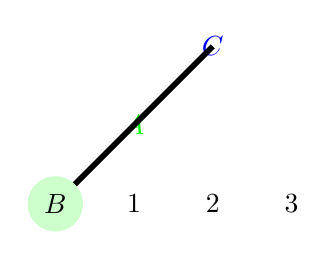
\begin{tikzpicture}
    % node语法:
    % \path node <for_loop> [<options>] (<name>) at (<coordinate>) :<animation_attribute>={<options>} {<node_content>}
    % 其中, for_loop/options/name/coordinate/animation_attribute都为可选, 并且顺序可打乱. 各参数效果如下:
    % 1.for_loop - 使用for循环作多个node
    % 2.options - 可指定node的各种属性. 可选列表如下:
    %   1)behind path | in front of path - 将node放置在当前path的下一层或上一层(默认)
    %   2)color - 边框颜色
    %   3)fill - 背景填充颜色
    %   4)draw - 给node增加边框
    %   5)line width - 边框宽度
    %   6)double - 边框使用双线
    %   7)shape - 指定背景形状,默认为矩形. 可选列表: 
    %     [1]circle - 圆
    %     [2]rectangle - 矩形
    %     下列需要使用shapes.geometric
    %     [3]ellipse - 椭圆
    %   8)inner sep - 文字与背景边框的距离, 默认为1/3em. 可使用以下参数分别指定x/y轴padding: inner xsep/inner ysep
    %   9)outer sep - 背景边框与外部内容的距离, 默认为line width的一半
    %   10)minimum height - 当文字高度和inner sep加起来小于指定值时,进行补足;当文字高度和inner sep加起来大于等于指定值时,不做改变
    %   11)minimum width - 类似于minimum height,用于宽度
    %   12)minimum size - 同时指定minimum height/width
    %   13)shape aspect - 宽度与高度的比率
    %   14)shape border rotate - 只有背景边框旋转,node内容不旋转,使用角度值指定
    %   15)text - 指定文本颜色,必须在color后面指定,不然会被color覆盖
    %   16)text opacity - 文本透明度
    %   17)align - 多行文本的对齐方式,文本使用\\主动换行,或根据text width参数值自动换行. 可选参数: 
    %     [1]left - 左对齐
    %     [2]flush left - 类似于左对齐,尽量避免分词,比left参数的右侧更错落有致
    %     [3]right - 右对齐
    %     [4]flush right - 类似于右对齐,尽量避免分词,比right参数的左侧更错落有致
    %     [5]center - 居中对齐
    %     [6]flush center - 类似于居中对齐,尽量避免分词,比center参数的两侧侧更错落有致
    %     [7]justify - 自动调整单词间隔,使两侧对齐
    %     [8]none - 不进行对齐
    %   18)text width - 文字所占宽度
    % 前提备注: node的中心位置默认在指定坐标处
    %   19)anchor - 坐标位于node内容的指定方位. 列表如下:
    %     [1]north - 坐标位于node内容的北侧
    %     [2]south - 坐标位于node内容的南侧
    %     [3]east - 坐标位于node内容的东侧
    %     [4]west - 坐标位于node内容的西侧
    %     [5]north east - 坐标位于node内容的东北侧
    %     [6]north west - 坐标位于node内容的西北侧
    %     [7]south east - 坐标位于node内容的东南侧
    %     [8]south west - 坐标位于node内容的西南侧
    %     [9]center - 坐标位于node内容的中心,默认值
    %   20)below - node内容相对于坐标的位置. 可用参数列表如下:
    %     [1]above - node内容位于坐标上方
    %     [2]below - node内容位于坐标下方
    %     [3]left - node内容位于坐标左方
    %     [4]right - node内容位于坐标右方
    %     [5]above left - node内容位于坐标左上方
    %     [6]above right - node内容位于坐标右上方
    %     [7]below left - node内容位于坐标左下方
    %     [8]below right - node内容位于坐标右下方
    %     [9]centered - node内容位于坐标位置
    %     备注: below/above/left/right可指定距离值;above left/above right/below left/below right也可指定距离值,并且可以使用<dimension_ver> and <dimension_hori>分别指定垂直距离和水平距离,但需要使用positioning库
    %   21)fit - 当前node的尺寸,可以容纳其他node,需要使用fit库. 格式: fit=(A)(B)(B)
    %   22)scale - 内容进行放大或缩小. 其他可使用的图形变化列表:
    %     [1]scale - 放大缩小
    %     [2]shift - 偏移
    %     [3]rotate - 旋转
    %   23)transform shape - 将外部的图形变化操作引入当前node
    %   24)pos - node在路径上(前一个坐标到当前坐标)的位置. 如: 0.5代表路径中点. 也可以使用如下参数:
    %     [1]at start - 类似于pos=0
    %     [2]very near start - 类似于pos=0.125
    %     [3]near start - 类似于pos=0.25
    %     [4]midway - 类似于pos=0.5
    %     [5]near end - 类似于pos=0.75
    %     [6]very near end - 类似于0.875
    %     [7]at end - 类似于pos=1
    %   25)auto - node相对于路径的位置. 可选列表: left/right
    %   26)swap - 相对于全局auto,当前环境内取auto的相反值
    %   27)sloped - 旋转文字,使文字顺着曲线的方向
    %   28)label - 在node处额外添加其他node. 格式: [<options>]<angle>:<text>. angle可选列表:
    %     [1]above/below/right/left/above left/above right/below left/below right
    %     [2]center - label node与主node的中心重合
    %     [3]角度值 - label的angle会偏向于45度的整数倍,无法精确定位角度
    %   29)pin - 类似于label,在主node与从node间添加连线
    % 3.name - node名称,便于后续引用
    % 4.at (<coordinate>) - node默认取用该关键字之前的最后一个坐标, 如果使用at (<coordinate>),则使用该坐标. 需要使用animations库
    % 5.:<animation_attribute>={<options>} - 配置关键帧属性,形成动画. 参考animate
    % 6.node_content - 文字实际内容,可以使用\includegraphics插入图片
    % 备注: \node为\path node的缩写形式
    \path node foreach \x in {1,2,3} at (\x,0) {\x};
    \path node (A) [color=green] at (1,1) {$A$};
    \draw[line width=2pt] (0,0) node[fill=green!20,shape=circle]{$B$} -- (2,2) node[behind path,color=blue]{$C$};
\end{tikzpicture}\\\vspace{1cm}

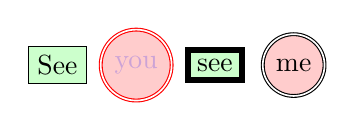
\begin{tikzpicture}
    % 配置所有node的属性
    [every node/.style={fill=green!20,draw},
    % 配置圆形背景node的属性
    every circle node/.style={fill=red!20,double}]
    \path node (A) at (0,0) {See};
    \path node[circle,color=red,text=blue,text opacity=0.2] (B) at (1,0) {you};
    \path node[line width=2pt] (C) at (2,0) {see};
    \path node[circle] (D) at (3,0) {me};
\end{tikzpicture}\\\vspace{1cm}

\begin{tikzpicture}
    % 配置锚点
    \path node[below=3pt,text=red] at (0,0) {I am here!};
    \path node[above left,text=blue] at (0,0) {I am here!};
    \path node[left,text=purple] at (0,0) {I am here!};
    \path node[below right=1cm and 5cm,text=orange] at (0,0) {I am here!};
    \fill[green!50] (0,0) circle [radius=1pt];
\end{tikzpicture}\\\vspace{1cm}

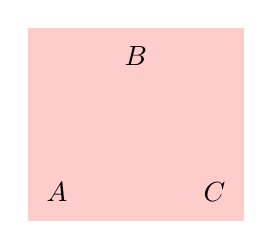
\begin{tikzpicture}
    % fit
    \path node (A) at (0,0) {$A$};
    \path node (B) at (1,1.732) {$B$};
    \path node (C) at (2,0) {$C$};
    \begin{scope}[on background layer]
      \path node[fill=red!20,shape=rectangle,fit=(A)(B)(C)] {}; 
    \end{scope}
\end{tikzpicture}\\\vspace{1cm}

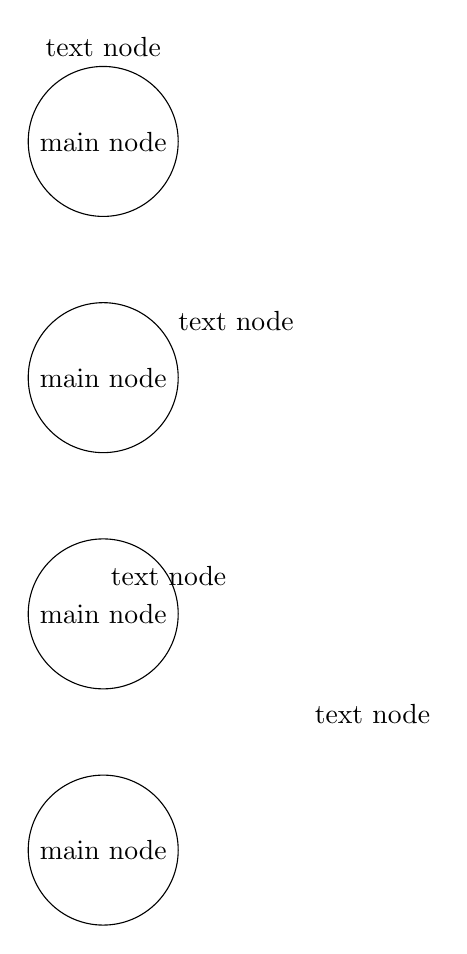
\begin{tikzpicture}
    % 其他node - label
    \path node[circle,draw,label=text node] (A) at (0,0) {main node};
    \path node[circle,draw,label=30:text node] (B) at (0,-3) {main node};
    \path node[circle,draw,label={[centered]30:text node}] (C) at (0,-6) {main node};
    \path node[circle,draw,label={[label distance=2cm]30:text node}] (D) at (0,-9) {main node};
\end{tikzpicture}
\end{document}
